\section{Numerical Integration}\label{sec:numerical_integration}

The Fundamental Theorem of Calculus gives a concrete technique for finding the exact value of a definite integral. That technique is based on computing antiderivatives. Despite the power of this theorem, there are still situations where we must \textit{approximate} the value of the definite integral instead of finding its exact value. The first situation we explore is where we \textit{cannot} compute an antiderivative of the integrand. The second case is when we actually do not know the integrand, but only its value when evaluated at certain points.\index{integration!numerical}\index{numerical integration} %While we handle both situations in the same way, we address them separately here.
%
%\subsection{An Antiderivative That Cannot Be Computed}
\bigskip

%\autoref{sec:antider} introduced antiderivatives and the indefinite integral; given a function, its indefinite integral is a set of \textit{functions}. In \autoref{sec:def_int}, we learned about definite integrals: given a function and two bounds, the definite integral computes the ``area under the curve,'' i.e., a \textit{number}. The Fundamental Theorem of Calculus states that these two concepts are related: we use antiderivatives to evaluate definite integrals. Definite integrals have immense importance in mathematics, science and engineering. We will explore some of these applications in \autoref{SEVEN}. 
%
%This method of evaluating definite integrals has one significant shortcoming: not all functions have an antiderivative expressible in terms of elementary functions.  (Elementary functions are combinations of polynomials, $n^{\text{th}}$ root, rational, exponential, logarithmic and trigonometric functions.). To be clear, we are not claiming that the antiderivatives are just \textit{hard} to find; rather, we are saying that we \textit{cannot} write them out using functions that we normally use. 
An \sword{elementary function}\index{elementary function} is any function that is a combination of polynomials, $n^{\text{th}}$ roots, rational, exponential, logarithmic and trigonometric functions and their inverses. We can compute the derivative of any elementary function, but there are many elementary functions of which we cannot compute an antiderivative. For example, the following functions do not have antiderivatives that we can express with elementary functions:
\[e^{-x^2}, \quad \sin(x^3)\quad \text{and} \quad \frac{\sin x}{x}.\]

The simplest way to refer to the antiderivatives of $e^{-x^2}$ is to simply write $\ds\int e^{-x^2}\ dx$. 

\mtable[-2in]{Graphically representing three definite integrals that cannot be evaluated using antiderivatives.}{fig:numerical1}{\begin{tikzpicture}
\begin{axis}[width=1.16\marginparwidth,tick label style={font=\scriptsize},
axis y line=middle,axis x line=middle,name=myplot,axis on top,
ymin=-.2,ymax=1.2,xmin=-.2,xmax=1.1]
\addplot[draw={\colorone},fill={\coloronefill},area style,domain=0:1]
 {exp(-x*x)}\closedcycle;
\draw (axis cs:.75,1) node {\scriptsize $y=e^{-x^2}$};
\end{axis}
\node [right] at (myplot.right of origin) {\scriptsize $x$};
\node [above] at (myplot.above origin) {\scriptsize $y$};
\end{tikzpicture}
\bigskip\\
\begin{tikzpicture}
\begin{axis}[width=1.16\marginparwidth,tick label style={font=\scriptsize},
axis y line=middle,axis x line=middle,name=myplot,axis on top,
ymin=-.6,ymax=1.2,xmin=-1,xmax=1.7]
\addplot[draw={\colorone},fill={\coloronefill},area style,domain=-pi/4:pi/2]
 {sin(deg(x^3))}\closedcycle;
\draw (axis cs:.6,.9) node {\scriptsize $y=\sin(x^3)$};
\end{axis}
\node [right] at (myplot.right of origin) {\scriptsize $x$};
\node [above] at (myplot.above origin) {\scriptsize $y$};
\end{tikzpicture}
\bigskip\\
\begin{tikzpicture}
\begin{axis}[width=1.16\marginparwidth,tick label style={font=\scriptsize},
axis y line=middle,axis x line=middle,name=myplot,axis on top,xtick={5,10,15},
ymin=-.3,ymax=1.1,xmin=-.9,xmax=15.9]
\addplot[draw={\colorone},fill={\coloronefill},area style,domain=.5:4*pi]
 {sin(deg(x))/x}\closedcycle;
\draw (axis cs:10,.7) node {\scriptsize $\displaystyle y=\frac{\sin x}{x}$};
\end{axis}
\node [right] at (myplot.right of origin) {\scriptsize $x$};
\node [above] at (myplot.above origin) {\scriptsize $y$};
\end{tikzpicture}}

%How, then, can we solve problems involving definite integrals of such functions? We \textit{approximate.} 
This section outlines three common methods of approximating the value of definite integrals. We describe each as a systematic method of approximating area under a curve. By approximating this area accurately, we find an accurate approximation of the corresponding definite integral.

We will apply the methods we learn in this section to the following definite integrals:
\[
 \int_0^1 e^{-x^2} \ dx, \quad
 \int_{-\frac{\pi}{4}}^{\frac{\pi}{2}} \sin(x^3) \ dx,
 \quad \text{and} \quad
 \int_{0.5}^{4\pi} \frac{\sin(x)}{x} \ dx,
\]
% todo Tim maybe use \pi/4 to \pi/2 in (b) instead?
as pictured in \autoref{fig:numerical1}.

\subsection{The Left and Right Hand Rule Methods}

In \autoref{sec:riemann} we addressed the problem of evaluating definite integrals by approximating the area under the curve using rectangles. We revisit those ideas here before introducing other methods of approximating definite integrals. \index{numerical integration!Left/Right Hand Rule}\index{Right Hand Rule}\index{Left Hand Rule}\index{integration!numerical!Left/Right Hand Rule}

We start with a review of notation. Let $f$ be a continuous function on the interval $[a,b]$. We wish to approximate $\ds \int_a^b f(x)\ dx$. We partition $[a,b]$ into $n$ equally spaced subintervals, each of length $\ds\Delta x = \frac{b-a}{n}$. The endpoints of these subintervals are labeled as
\[x_0=a,\ x_1 = a+\Delta x,\ x_2 = a+ 2\Delta x,\ \dotsc,\ x_i = a+i\Delta x,\ \dotsc,\ x_n = b.\]

%\autoref{idea:riemann}
\autoref{sec:riemann} showed that to use the Left Hand Rule we use the summation $\ds \sum_{i=1}^n f(x_{i-1})\Delta x$ and to use the Right Hand Rule we use $\ds \sum_{i=1}^n f(x_i)\Delta x$. We review the use of these rules in the context of examples.

\example{ex_num1}{Approximating definite integrals with rectangles}{Approximate $\ds \int_0^1e^{-x^2}\ dx$ using the Left and Right Hand Rules with 5 equally spaced subintervals.}
{We begin by partitioning the interval $[0,1]$ into 5 equally spaced intervals. We have $\Delta x = \frac{1-0}5 = 1/5=0.2$, so
\[x_0=0,\ x_1=0.2,\ x_2=0.4,\ x_3=0.6,\ x_4=0.8,\text{ and }x_5=1.\]

\mtable{Approximating $\ds\int_0^1e^{-x^2}\ dx$ in \autoref{ex_num1} using (top) the left hand rule and (bottom) the right hand rule.}{fig:num1}{\begin{tikzpicture}
\begin{axis}[width=1.16\marginparwidth,tick label style={font=\scriptsize},
axis y line=middle,axis x line=middle,name=myplot,axis on top,xtick={.2,.4,.6,.8,1},
ymin=-.2,ymax=1.2,xmin=-.2,xmax=1.1]
\addplot[draw={\colorone},fill={\coloronefill},area style,domain=0:1]
 {exp(-x*x)}\closedcycle;
\foreach \x in {0,0.2,...,.8} {
 \edef\y{exp(-\x*\x)}
 \edef\temp{\noexpand\draw[thick,draw={\colortwo}]
  (axis cs:\x,0)rectangle(axis cs:{\x+.2},{\y});
 }\temp
}
\draw (axis cs:.75,1) node {\scriptsize $y=e^{-x^2}$};
\end{axis}
\node [right] at (myplot.right of origin) {\scriptsize $x$};
\node [above] at (myplot.above origin) {\scriptsize $y$};
\end{tikzpicture}
\bigskip\\
\begin{tikzpicture}
\begin{axis}[width=1.16\marginparwidth,tick label style={font=\scriptsize},
axis y line=middle,axis x line=middle,name=myplot,axis on top,xtick={.2,.4,.6,.8,1},
ymin=-.2,ymax=1.2,xmin=-.2,xmax=1.1]
\addplot[draw={\colorone},fill={\coloronefill},area style,domain=0:1]
 {exp(-x*x)}\closedcycle;
\foreach \x in {0.2,0.4,...,1} {
 \edef\y{exp(-\x*\x)}
 \edef\temp{\noexpand\draw[thick,draw={\colortwo}]
  (axis cs:\x,0)rectangle(axis cs:{\x-.2},{\y});
 }\temp
}
\draw (axis cs:.75,1) node {\scriptsize $y=e^{-x^2}$};
\end{axis}
\node [right] at (myplot.right of origin) {\scriptsize $x$};
\node [above] at (myplot.above origin) {\scriptsize $y$};
\end{tikzpicture}}

Using the Left Hand Rule, we have:
\begin{align*}
	\sum_{i=1}^n f(x_{i-1})\Delta x
	&= \big(f(x_0)+f(x_1)+f(x_2) + f(x_3) + f(x_4)\big)\Delta x \\
	&= \big(f(0) + f(0.2) + f(0.4) + f(0.6) + f(0.8)\big)\Delta x \\
	&\approx \big(1+0.961 + 0.852 + 0.698 + 0.527)(0.2)\\
	&\approx 0.808.
\end{align*}

Using the Right Hand Rule, we have:
\begin{align*}
	\sum_{i=1}^n f(x_i)\Delta x
	&= \big(f(x_1)+f(x_2) + f(x_3) + f(x_4) + f(x_5)\big)\Delta x \\
	&= \big(f(0.2) + f(0.4) + f(0.6) + f(0.8)+f(1)\big)\Delta x \\
	&\approx \big(0.961 +0.852 + 0.698 + 0.527 + 0.368)(0.2)\\
	&\approx 0.681.
\end{align*}

\autoref{fig:num1} shows the rectangles used in each method to approximate the definite integral. These graphs show that in this particular case, the Left Hand Rule is an over approximation and the Right Hand Rule is an under approximation. To get a better approximation, we could use more rectangles, as we did in \autoref{sec:riemann}. We could also average the Left and Right Hand Rule results together, giving
\[\frac{0.808 + 0.681}{2} = 0.7445.\]
The actual answer, accurate to 4 places after the decimal, is 0.7468, showing our average is a good approximation.}

\mtable[-.5in]{Table of values used to approximate $\ds\int_{-\frac{\pi}4}^{\frac{\pi}2}\sin(x^3)\ dx$ in \autoref{ex_num2}.}{fig:num2a}{%
	\begin{tabular}{lrll}\lxBeginTableHead
	$x_i$ & Exact & Approx. & $\sin(x_i^3)$ \\\lxEndTableHead\midrule
	$x_0$ & $-\pi/4\phantom{0}$ & $-0.785$ & $-0.466$ \\
	$x_1$ & $-7\pi/40$ & $-0.550$ & $-0.165$ \\
	$x_2$ & $-\pi/10$ & $-0.314$ & $-0.031$ \\
	$x_3$ & $-\pi/40$ & $-0.0785$ & $\phantom{-}0$ \\
	$x_4$ & $\pi/20$ & $\phantom{-}0.157$ & $\phantom{-}0.004$ \\
	$x_5$ & $\pi/8\phantom{0}$ & $\phantom{-}0.393$ & $\phantom{-}0.061$ \\
	$x_6$ & $\pi/5\phantom{0}$ & $\phantom{-}0.628$ & $\phantom{-}0.246$ \\
	$x_7$ & $11\pi/40$ & $\phantom{-}0.864$ & $\phantom{-}0.601$ \\
	$x_8$ & $7\pi/20$ & $\phantom{-}1.10$ & $\phantom{-}0.971$ \\
	$x_9$ & $17\pi/40$ & $\phantom{-}1.34$ & $\phantom{-}0.690$ \\
	$x_{10}$ & $\pi/2\phantom{0}$ & $\phantom{-}1.57$ & $-0.670$
\end{tabular}}

\example{ex_num2}{Approximating definite integrals with rectangles}{Approximate $\ds\int_{-\frac{\pi}4}^{\frac{\pi}2} \sin (x^3)\ dx$ using the Left and Right Hand Rules with 10 equally spaced subintervals.}
{We begin by finding $\Delta x$:
\[\frac{b-a}{n} = \frac{\pi/2 - (-\pi/4)}{10} = \frac{3\pi}{40}\approx 0.236.\]
It is useful to write out the endpoints of the subintervals in a table; in \autoref{fig:num2a}, we give the exact values of the endpoints, their decimal approximations, and decimal approximations of $\sin(x^3)$ evaluated at these points. 

\mtable{Approximating\\ $\ds\int_{-\frac{\pi}4}^{\frac{\pi}2}\sin(x^3)\ dx$ in \autoref{ex_num2} using (top) the left hand rule and (bottom) the right hand rule.}{fig:num2b}{%
\begin{tikzpicture}
\begin{axis}[width=1.16\marginparwidth,tick label style={font=\scriptsize},
axis y line=middle,axis x line=middle,name=myplot,axis on top,
ymin=-.7,ymax=1.2,xmin=-1,xmax=1.7]
\addplot[draw={\colorone},fill={\coloronefill},area style,domain=-pi/4:pi/2]
 {sin(deg(x^3))}\closedcycle;
\foreach \x / \y in %
                {-0.785/ -0.466, -0.550/-0.165, -0.314/ -0.0310,%
                 -0.0785/-0.000484, 0.157/ 0.00388, 0.393/ 0.0605,
                 0.628/ 0.246, 0.864/ 0.601, 1.10/ 0.971, 1.34/ 0.690} {
 \addplot [thick,draw={\colortwo}] coordinates
  {(\x+.2356,0) (\x+.2356,\y) (\x,\y) (\x,0) (\x+.2356,0)};
}
\draw (axis cs:.6,.9) node {\scriptsize $y=\sin(x^3)$};
\end{axis}
\node [right] at (myplot.right of origin) {\scriptsize $x$};
\node [above] at (myplot.above origin) {\scriptsize $y$};
\end{tikzpicture}
\\
\begin{tikzpicture}
\begin{axis}[width=1.16\marginparwidth,tick label style={font=\scriptsize},
axis y line=middle,axis x line=middle,name=myplot,axis on top,
ymin=-.7,ymax=1.2,xmin=-1,xmax=1.7]
\addplot[draw={\colorone},fill={\coloronefill},area style,domain=-pi/4:pi/2]
 {sin(deg(x^3))}\closedcycle;
\foreach \x / \y in %
               {-0.550/-0.165, -0.314/ -0.0310,%
                -0.0785/-0.000484, 0.157/ 0.00388, 0.393/ 0.0605,
                0.628/ 0.246, 0.864/ 0.601, 1.10/ 0.971, 1.34/ 0.690, 1.57/ -0.670} {
  \addplot [thick,draw={\colortwo}] coordinates
    {(\x-.2356,0) (\x-.2356,\y) (\x,\y) (\x,0) (\x-.2356,0)};
}
\draw (axis cs:.6,1.1) node {\scriptsize $y=\sin(x^3)$};
\end{axis}
\node [right] at (myplot.right of origin) {\scriptsize $x$};
\node [above] at (myplot.above origin) {\scriptsize $y$};
\end{tikzpicture}}

Once this table is created, it is straightforward to approximate the definite integral using the Left and Right Hand Rules. (Note: the table itself is easy to create, especially with a standard spreadsheet program on a computer. The last two columns are all that are needed.) The Left Hand Rule sums the first 10 values of $\sin(x_i^3)$ and multiplies the sum by $\Delta x$; the Right Hand Rule sums the last 10 values of $\sin(x_i^3)$ and multiplies by $\Delta x$. Therefore we have:
\begin{align*}
	\text{Left Hand Rule: }\int_{-\frac{\pi}4}^{\frac{\pi}2}\sin(x^3)\ dx
	& \approx (1.91)(0.236) = 0.451. \\
	\text{Right Hand Rule: }\int_{-\frac{\pi}4}^{\frac{\pi}2}\sin(x^3)\ dx
	&\approx (1.71)(0.236) = 0.404.
\end{align*}

The average of the Left and Right Hand Rules is 0.4275.  The actual answer, accurate to 3 places after the decimal, is 0.460. Our approximations were once again fairly good. The rectangles used in each approximation are shown in \autoref{fig:num2b}. It is clear from the graphs that using more rectangles (and hence, narrower rectangles) should result in a more accurate approximation.}

\subsection{The Trapezoidal Rule}

In \autoref{ex_num1} we approximated the value of $\ds \int_0^1 e^{-x^2}\ dx$ with 5 rectangles of equal width. \autoref{fig:num1} showed the rectangles used in the Left and Right Hand Rules. These graphs clearly show that rectangles do not match the shape of the graph all that well, and that accurate approximations will only come by using lots of rectangles. \index{Trapezoidal Rule}\index{numerical integration!Trapezoidal Rule}\index{integration!numerical!Trapezoidal Rule}

\mtable{Approximating $\int_0^1 e^{-x^2}\ dx$ using 5 trapezoids of equal widths.}{fig:num3a}{\begin{tikzpicture}
\begin{axis}[width=1.16\marginparwidth,tick label style={font=\scriptsize},
axis y line=middle,axis x line=middle,name=myplot,axis on top,xtick={.2,.4,...,1},
ymin=-.2,ymax=1.2,xmin=-.2,xmax=1.1]
\addplot[draw={\colorone},fill={\coloronefill},area style,domain=0:1]
 {exp(-x*x)}\closedcycle;
\foreach\x in{0,.2,...,.8}{
  \edef\y{{exp(-\x*\x)}}
  \edef\z{{exp(-(\x+.2)*(\x+.2))}}
  \edef\temp{\noexpand\addplot[thick,draw={\colortwo}] coordinates
   {(\x,0) (\x,\y) ({\x+.2},\z) ({\x+.2},0) (\x,0)};
 }\temp
}
\draw (axis cs:.75,1) node {\scriptsize $y=e^{-x^2}$};
\end{axis}
\node [right] at (myplot.right of origin) {\scriptsize $x$};
\node [above] at (myplot.above origin) {\scriptsize $y$};
\end{tikzpicture}}

Instead of using rectangles to approximate the area, we can instead use \textit{trapezoids.} In \autoref{fig:num3a}, we show the region under $f(x) = e^{-x^2}$ on $[0,1]$ approximated with 5 trapezoids of equal width; the top ``corners'' of each trapezoid lie on the graph of $f(x)$. It is clear from this figure that these trapezoids more accurately approximate the area under $f$ and hence should give a better approximation of $\int_0^1 e^{-x^2}\ dx$. (In fact, these trapezoids seem to give a \textit{great} approximation of the area.)

\youtubeVideo{8z6JRFvjkpc}{The Trapezoid Rule for Approximating Integrals}

\mtable{The area of a trapezoid is $\frac{a+b}2h$.}{fig:trapezoid}{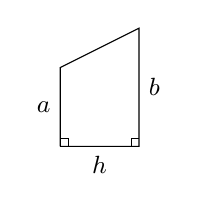
\begin{tikzpicture}
\draw(0,0)--node[pos=.5,left]{\small $a$}(0,1)--(1,1.5)
 --node[pos=.5,right]{\small$b$}(1,0)--node[pos=.5,below]{\small$h$}(0,0);
\draw(0,.1)--(.1,.1)--(.1,0);
\draw(.9,0)--(.9,.1)--(1,.1);
%\draw(2.5,.75)node{Area = };
\end{tikzpicture}}

The formula for the area of a trapezoid is given in \autoref{fig:trapezoid}. We approximate $\int_0^1 e^{-x^2}\ dx$ with these trapezoids in the following example.

\example{ex_num3}{Approximating definite integrals using trapezoids}{Use 5 trapezoids of equal width to approximate $\ds \int_0^1e^{-x^2}\ dx$.}
{To compute the areas of the 5 trapezoids in \autoref{fig:num3a}, it will again be useful to create a table of values as shown in \autoref{fig:num3b}.

\mtable{A table of values of $e^{-x^2}$.}{fig:num3b}{%
\begin{tabular}{ll}\lxBeginTableHead
$x_i$ & $e^{-x_i^2}$ \\\lxEndTableHead\midrule
0 & 1\\
0.2 & 0.961 \\
0.4 & 0.852 \\
0.6 & 0.698 \\
0.8 & 0.527 \\
1 & 0.368
\end{tabular}}

The leftmost trapezoid has legs of length 1 and 0.961 and a height of 0.2. Thus, by our formula, the area of the leftmost trapezoid is:
\[\frac{1+0.961}{2}(0.2) = 0.1961.\]
Moving right, the next trapezoid has legs of length 0.961 and 0.852 and a height of 0.2. Thus its area is:
\[\frac{0.961+0.852}2(0.2) = 0.1813.\]

The sum of the areas of all 5 trapezoids is:
\begin{align*}
\frac{1+0.961}{2}(0.2) + \frac{0.961+0.852}2(0.2)+\frac{0.852+0.698}2(0.2)& \\
+\frac{0.698+0.527}2(0.2)+\frac{0.527+0.368}2(0.2)&= 0.7445.
\end{align*}
We approximate $\ds \int_0^1 e^{-x^2}\ dx \approx 0.7445.$}

There are many things to observe in this example. Note how each term in the final summation was multiplied by both 1/2 and by $\Delta x = 0.2$. We can factor these coefficients out, leaving a more concise summation as:\\
\flushinnerequ{\small
\[
\frac12(0.2)\Big[(1+0.961) + (0.961+0.852) + (0.852+0.698) + ( 0.698+ 0.527) +(0.527 + 0.368)\Big].
\]}\\
Now notice that all numbers except for the first and the last are added twice. Therefore we can write the summation even more concisely as
\[\frac{0.2}{2}\Big[1 + 2(0.961+0.852+0.698+0.527) + 0.368\Big].\]

This is the heart of the \textbf{Trapezoidal Rule}, wherein a definite integral $\ds \int_a^b f(x) \ dx$ is approximated by using trapezoids of equal widths to approximate the corresponding area under $f$. Using $n$ equally spaced subintervals with endpoints $x_0$, $x_1$, \dots, $x_n$, we again have $\ds \Delta x = \frac{b-a}n$. Thus:
\begin{align*}
	\int_a^b f(x)\ dx
	& \approx \sum_{i=1}^n \frac{f(x_{i-1})+f(x_i)}2\Delta x \\
	& = \frac{\Delta x}2 \sum_{i=1}^n \big(f(x_{i-1})+f(x_i)\big)\\
	& = \frac{\Delta x}2\left[f(x_0)+ 2\sum_{i=1}^{n-1} f(x_i) + f(x_n)\right].
\end{align*}

\example{ex_num4}{Using the Trapezoidal Rule}{Revisit \autoref{ex_num2} 
and approximate $\ds\int_{-\frac{\pi}{4}}^{\frac{\pi}{2}} \sin (x^3)\ dx$ using the Trapezoidal Rule and 10 equally spaced subintervals.}
{We refer back to \autoref{fig:num2a} for the table of values of $\sin(x^3)$. Recall that $\Delta x = 3\pi/40 \approx 0.236$. Thus we have:\small
\begin{align*}
	\int_{-\frac{\pi}4}^{\frac{\pi}2} & \sin (x^3)\ dx \\
	&\approx \frac{0.236}{2}\Big[-0.466 + 2\Big(-0.165+(-0.031)+\dotsb+%0.971+
0.69\Big)+(-0.67)\Big]\\
	&= 0.4275.\eoehere
\end{align*}
\normalsize}

Notice how ``quickly'' the Trapezoidal Rule can be implemented once the table of values is created. This is true for all the methods explored in this section; the real work is creating a table of $x_i$ and $f(x_i)$ values. Once this is completed, approximating the definite integral is not difficult. Again, using technology is wise. Spreadsheets can make quick work of these computations and make using lots of subintervals easy. 

Also notice the  approximations the Trapezoidal Rule gives. It is  the average of the approximations given by the Left and Right Hand Rules! This effectively renders the Left and Right Hand Rules obsolete. They are useful when first learning about definite integrals, but if a real approximation is needed, one is generally better off using the Trapezoidal Rule instead of either the Left or Right Hand Rule.

We will also show that the Trapezoidal Rule makes using the Midpoint Rule obsolete as well.  With much more work, it will turn out that the Midpoint Rule has only a marginal gain in accuracy.  But we will include it in our results for the sake of completeness.\bigskip

How can we improve on the Trapezoidal Rule, apart from using more and more trapezoids? The answer is clear once we look back and consider what we have \textit{really} done so far. The Left Hand Rule is not \textit{really} about using rectangles to approximate area. Instead, it approximates a function $f$ with constant functions on small subintervals and then computes the definite integral of these constant functions. The Trapezoidal Rule is really approximating a function $f$ with a linear function on a small subinterval, then computes the definite integral of this linear function. In both of these cases the definite integrals are easy to compute in geometric terms.

So we have a progression: we start by approximating $f$ with a constant function and then with a linear function. What is next? A quadratic function. By approximating the curve of a function with lots of parabolas, we generally get an even better approximation of the definite integral. We call this process \textbf{Simpson's Rule}, named after Thomas Simpson (1710-1761), even though others had used this rule as much as 100 years prior.

\subsection{Simpson's Rule}

Given one point, we can create a constant function that goes through that point. Given two points, we can create a linear function that goes through those points. Given three points, we can create a quadratic function that goes through those three points (given that no two have the same $x$-value).\index{Simpson's Rule}\index{numerical integration!Simpson's Rule}\index{integration!numerical!Simpson's Rule}

Consider three points $(x_1,y_1)$, $(x_2,y_2)$ and $(x_3,y_3)$ whose $x$-values are equ\-ally spaced and $x_1<x_2<x_3$. Let $f$ be the quadratic function that goes through these three points. An exercise will ask you to show that 
\begin{equation}
\int_{x_1}^{x_3} f(x)\ dx = \frac{x_3-x_1}{6}\big(y_1+4y_2+y_3\big).\label{eq:simpsons}
\end{equation}

\mtable{A graph of a function $f$ and a parabola that approximates it well on $[1,3]$.}{fig:numsimpsons}{\begin{tikzpicture}
\begin{axis}[width=1.16\marginparwidth,tick label style={font=\scriptsize},
axis y line=middle,axis x line=middle,name=myplot,axis on top,xtick={1,2,3},
ytick={1,2,3},ymin=-.2,ymax=4,xmin=.5,xmax=3.5]
\addplot [draw={\colorone},domain=.9:3.1,thick] {11-12*x+4.5*x^2-.5*x^3};
\addplot [draw={\colortwo},dashed,domain=.9:3.1,thick] {8-6.5*x+1.5*x^2};
\filldraw (axis cs:1,3) circle (1pt);
\filldraw (axis cs:2,1) circle (1pt);
\filldraw (axis cs:3,2) circle (1pt);
\end{axis}
\node [right] at (myplot.right of origin) {\scriptsize $x$};
\node [above] at (myplot.above origin) {\scriptsize $y$};
\end{tikzpicture}}

Consider \autoref{fig:numsimpsons}. A function $f$ goes through the 3 points shown and the parabola $g$ that also goes through those points is graphed with a dashed line. Using our equation from above, we know exactly that
\[\int_1^3 g(x) \ dx = \frac{3-1}{6}\big(3+4(1)+2\big)= 3.\]
Since $g$ is a good approximation for $f$ on $[1,3]$, we can state that
\[\int_1^3 f(x)\ dx \approx 3.\]

Notice how the interval $[1,3]$ was split into two subintervals as we needed 3 points. Because of this, whenever we use Simpson's Rule, we need to break the interval into an even number of subintervals. 

In general, to approximate $\ds \int_a^b f(x)\ dx$ using Simpson's Rule, subdivide $[a,b]$ into $n$ subintervals, where $n$ is even and each subinterval has width $\Delta x = (b-a)/n$. We approximate $f$ with $n/2$ parabolic curves, using \autoeqref{eq:simpsons} to compute the area under these parabolas. Adding up these areas gives the formula:
\begin{multline*}
\int_a^b f(x) \ dx\approx\\
\frac{\Delta x}3
\left[f(x_0)+4f(x_1)+2f(x_2)+4f(x_3)+\dotsb+2f(x_{n-2})+4f(x_{n-1})+f(x_n)\right].
\end{multline*}
Note how the coefficients of the terms in the summation have the pattern 1, 4, 2, 4, 2, 4, \dots, 2, 4, 1.

Let's demonstrate Simpson's Rule with a concrete example.

\example{ex_num5}{Using Simpson's Rule}{Approximate $\ds\int_0^1 e^{-x^2}\ dx$ using Simpson's Rule and 4 equally spaced subintervals.}
{We begin by making a table of values as we have in the past, as shown in \autoref{fig:num5a}(a). Simpson's Rule states that
\mtable{A table of values to approximate $\int_0^1e^{-x^2}\ dx$ in \autoref{ex_num5}, along with a graph of the function.}{fig:num5a}{%
\begin{tabular}{ll}\lxBeginTableHead
$x_i$ & $e^{-x_i^2}$ \\\lxEndTableHead\midrule
0 & 1 \\
0.25 & 0.939 \\
0.5 & 0.779 \\
0.75 & 0.570 \\
1 & 0.368
\end{tabular}
\\ (a) \\
\begin{tikzpicture}
\begin{axis}[width=1.16\marginparwidth,tick label style={font=\scriptsize},
axis y line=middle,axis x line=middle,name=myplot,axis on top,xtick={.25,.5,.75,1},
ymin=-.2,ymax=1.2,xmin=-.2,xmax=1.1]
\addplot[draw={\colorone},fill={\coloronefill},area style,domain=0:1]
 {exp(-x*x)}\closedcycle;
\addplot [draw={\colortwo},domain=0:.5,thick] {1-0.042*x-0.8*x^2};
\addplot [draw={\colortwo},domain=.5:1,thick] {1.218-0.907*x+0.0569*x^2};
\addplot [thick,draw={\colortwo}] coordinates {(0,1) (0,0) (.5,0) (.5,.779)};
\addplot [thick,draw={\colortwo}] coordinates {(.5,0) (1,0) (1,.368)};
\draw (axis cs:.75,1) node {\scriptsize $y=e^{-x^2}$};
\filldraw (axis cs:0,1) circle (1pt)
          (axis cs:.25,.939) circle (1pt)
          (axis cs:.5,.779) circle (1pt)
          (axis cs:.75,.57) circle (1pt)
          (axis cs:1,.368) circle (1pt);
\end{axis}
\node [right] at (myplot.right of origin) {\scriptsize $x$};
\node [above] at (myplot.above origin) {\scriptsize $y$};
\end{tikzpicture}
\\ (b)}
\[
 \int_0^1e^{-x^2}\ dx
 \approx \frac{0.25}{3}\Big[1+4(0.939)+2(0.779)+4(0.570) + 0.368\Big]
 = 0.7468\overline{3}.
\]

Recall in \autoref{ex_num1} we stated that the correct answer, accurate to 4 places after the decimal, was 0.7468. Our approximation with Simpson's Rule, with 4 subintervals, is better than our approximation with the Trapezoidal Rule using 5.

\autoref{fig:num5a}(b) shows $f(x) = e^{-x^2}$ along with its approximating parabolas, demonstrating how good our approximation is. The approximating curves are nearly indistinguishable from the actual function.}

\example{ex_num6}{Using Simpson's Rule}{Approximate $\ds\int_{-\frac{\pi}4}^{\frac{\pi}2} \sin (x^3)\ dx$ using Simpson's Rule and 10 equally spaced intervals.}
{\mtable{A table of values to approximate $\int_{-\frac{\pi}4}^{\frac{\pi}2}\sin(x^3)\ dx$ in \autoref{ex_num6}, along with a graph of the function.}{fig:num6a}{%
\begin{tabular}{ll}\lxBeginTableHead
  $x_i$ & $\sin(x_i^3)$ \\\lxEndTableHead\midrule
  $-0.785$ & $-0.466$ \\
  $-0.550$ & $-0.165$   \\
  $-0.314$ & $-0.031$ \\
  $-0.0785$ & $\phantom{-}0$   \\
  $\phantom{-}0.157$ & $\phantom{-}0.004$ \\
  $\phantom{-}0.393$ & $\phantom{-}0.061$ \\
  $\phantom{-}0.628$ & $\phantom{-}0.246$ \\
  $\phantom{-}0.864$ & $\phantom{-}0.601$ \\
  $\phantom{-}1.10$ & $\phantom{-}0.971$ \\
  $\phantom{-}1.34$ & $\phantom{-}0.690$ \\
  $\phantom{-}1.57$ & $-0.670$ \\
\end{tabular}
\\ (a) \\
\begin{tikzpicture}
\begin{axis}[width=1.16\marginparwidth,tick label style={font=\scriptsize},
axis y line=middle,axis x line=middle,name=myplot,axis on top,
ymin=-.7,ymax=1.2,xmin=-1,xmax=1.7]
\addplot[draw={\colorone},fill={\coloronefill},area style,domain=-pi/4:pi/2]
 {sin(deg(x^3))}\closedcycle;
\addplot [draw={\colortwo},domain=-.785:-.314,thick] {-.11-.721*x-1.49*x^2};
\addplot [thick,draw={\colortwo}] coordinates {(-.785,-.466) (-.785,0) (-.314,0) (-.314,-.03)};
\addplot [draw={\colortwo},domain=-.314:.157,thick] {.004+.037*x-.236*x^2};
\addplot [thick,draw={\colortwo}] coordinates {(-.314,0) (.157,0) (.157,.004)};
\addplot [draw={\colortwo},domain=.157:.628,thick] {.037-.395*x+1.156*x^2};
\addplot [thick,draw={\colortwo}] coordinates {(.157,0) (.628,0) (.628,.246)};
\addplot [draw={\colortwo},domain=.628:1.1,thick] {-.632+1.32*x+.13*x^2};
\addplot [thick,draw={\colortwo}] coordinates {(.628,0) (1.1,0) (1.1,.971)};
\addplot [draw={\colortwo},domain=1.1:1.57,thick] {-11.98+22.46*x-9.72*x^2};
\addplot [thick,draw={\colortwo}] coordinates {(1.1,0) (1.57,0) (1.57,-.67)};
\filldraw (axis cs:-.785,-.466 ) circle (1pt)
          (axis cs:-.55,-.165 ) circle (1pt)
          (axis cs:-.314,-.031 ) circle (1pt)
          (axis cs:-.0785,0 ) circle (1pt)
          (axis cs:.157,.004 ) circle (1pt)
          (axis cs:.393,.061 ) circle (1pt)
          (axis cs:.628,.246 ) circle (1pt)
          (axis cs:.864,.601 ) circle (1pt)
          (axis cs:1.1,.971 ) circle (1pt)
          (axis cs:1.34,.69 ) circle (1pt)
          (axis cs:1.57,-.67 ) circle (1pt);
\draw (axis cs:.6,.9) node {\scriptsize $y=\sin(x^3)$};
\end{axis}
\node [right] at (myplot.right of origin) {\scriptsize $x$};
\node [above] at (myplot.above origin) {\scriptsize $y$};
\end{tikzpicture}
\\ (b)}%
\autoref{fig:num6a}(a) shows the table of values that we used in the past for this problem, shown here again for convenience. Again, $\Delta x = (\pi/2+\pi/4)/10 \approx 0.236$.

Simpson's Rule states that
{\small\begin{align*}
	\int_{-\frac{\pi}4}^{\frac{\pi}2} \sin (x^3)\ dx
	&\approx \frac{0.236}3\Big[(-0.466)+4(-0.165)+2(-0.031) + \dotsb \\
	&\qquad\qquad \dotsb + 2(0.971) + 4(0.69) + (-0.67)\Big]\\
	&= 0.4701
\end{align*}}

Recall that the actual value, accurate to 3 decimal places, is 0.460. Our approximation is within one 1/100$^\text{th}$ of the correct value. The graph in \autoref{fig:num6a}(b) shows how closely the parabolas match the shape of the graph.}

%\noindent\begin{minipage}[t]{\linewidth}\noindent%
%\captionsetup{type=figure}%
%
%\caption{Approximating $\int_{-\frac{\pi}4}^{\frac{\pi}2}\sin(x^3)\ dx$ in \autoref{ex_num6} with Simpson's Rule and 10 equally spaced intervals.}
%\label{fig:num6b}
%\end{minipage}

\subsection{Summary and Error Analysis}

We summarize the key concepts of this section thus far in the following Key Idea.

{
\tcbset{grow to right by=140pt}
\begin{keyidea}[Numerical Integration]\label{idea:numerical}
Let $f$ be a continuous function on $[a,b]$, let $n$ be a positive integer, and let $\ds\Delta x = \frac{b-a}{n}$.
Set $x_0=a$, $x_1=a+\Delta x$, \dots, $x_i = a+i\Delta x$, $x_n=b$.
Consider $\ds\int_a^b f(x)\ dx$.\\
\index{integration!numerical!Left Hand Rule}
\index{integration!numerical!Right Hand Rule}
\index{integration!numerical!Midpoint Rule}
\index{integration!numerical!Trapezoidal Rule}
\index{integration!numerical!Simpson's Rule}
\index{Left/Right Hand Rule}\index{Midpoint Rule}
\index{Trapezoidal Rule}\index{Simpson's Rule}
\index{numerical integration!Left Hand Rule}
\index{numerical integration!Right Hand Rule}
\index{numerical integration!Midpoint Rule}
\index{numerical integration!Trapezoidal Rule}
\index{numerical integration!Simpson's Rule}
\begin{tabular}{ll}
Left Hand Rule: &
$\ds\int_a^b f(x)\ dx \approx \Delta x\Big[f(x_0) + f(x_1) + \dotsb + f(x_{n-1})\big]$.\\
Right Hand Rule: &
$\ds\int_a^b f(x)\ dx \approx \Delta x\Big[f(x_1) + f(x_2) + \dotsb + f(x_n)\big]$.\\
Midpoint Rule: &
$\ds\int_a^b f(x)\ dx \approx \Delta x\Big[f\big(\frac{x_0+x_1}2\big) + f\big(\frac{x_1+x_2}2\big) + \dotsb + f\big(\frac{x_{n-1}+x_n}2\big)\big]$.\\
Trapezoidal Rule: &
$\ds\int_a^b f(x)\ dx \approx \frac{\Delta x}2\Big[f(x_0) + 2f(x_1) + 2f(x_2) +\dotsb + 2f(x_{n-1})+ f(x_n)\big]$.\\
Simpson's Rule: &
$\ds\int_a^b f(x)\ dx \approx \frac{\Delta x}3\Big[f(x_0) + 4f(x_1) + 2f(x_2) +\dotsb + 4f(x_{n-1})+ f(x_n)\big]$ {\small ($n$ even)}.
\end{tabular}
\end{keyidea}
}

In our examples, we approximated the value of a definite integral using a given method then compared it to the ``right'' answer. This should have raised several questions in the reader's mind, such as:
\begin{enumerate}
	\item	How was the ``right'' answer computed?
	\item	If the right answer can be found, what is the point of approximating?
	\item	If there is value to approximating, how are we supposed to know if the approximation is any good?
\end{enumerate}

These are good questions, and their answers are educational. In the examples, \textit{the} right answer was never computed. Rather, an approximation accurate to a certain number of places after the decimal was given. In \autoref{ex_num1}, we do not know the \textit{exact} answer, but we know it starts with 0.7468. These more accurate approximations were computed using numerical integration but with more precision (i.e., more subintervals and the help of a computer). 

Since the exact answer cannot be found, approximation still has its place. How are we to tell if the approximation is any good?

``Trial and error'' provides one way. %(No, this does not refer to seeing whether or not the bridge collapses.) 
Using technology, make an approximation with, say, 10, 100, and 200 subintervals. This likely will not take much time at all, and a trend should emerge. If a trend does not emerge, try using yet more subintervals. Keep in mind that trial and error is never foolproof; you might stumble upon a problem in which a trend will not emerge.

A second method is to use Error Analysis. While the details are beyond the scope of this text, there are some formulas that give \textit{bounds} for how good your approximation will be. For instance, the formula might state that the approximation is within 0.1 of the correct answer. If the approximation is 1.58, then one knows that the correct answer is between 1.48 and 1.68. By using lots of subintervals, one can get an approximation as accurate as one likes. \autoref{thm:numerical_error} states what these bounds are.

\begin{theorem}[Error Bounds in Numerical Integration]\label{thm:numerical_error}
Suppose that $M_n$ is an upper bound on $\abs{f^{(n)}(x)}$ on $[a,b]$.  Then a bound for the error of the numerical method of integration is given by:
\index{integration!numerical!Left Hand Rule}
\index{integration!numerical!Right Hand Rule}
\index{integration!numerical!Midpoint Rule}
\index{integration!numerical!Trapezoidal Rule}
\index{integration!numerical!Simpson's Rule}
\index{Left/Right Hand Rule!error bounds}
\index{Midpoint Rule!error bounds}
\index{Trapezoidal Rule!error bounds}
\index{Simpson's Rule!error bounds}
\index{numerical integration!Left Hand Rule!error bounds}
\index{numerical integration!Right Hand Rule!error bounds}
\index{numerical integration!Midpoint Rule!error bounds}
\index{numerical integration!Trapezoidal Rule!error bounds}
\index{numerical integration!Simpson's Rule!error bounds}
\begin{center}
\begin{tabular}{lc}
Method & Error Bound \\\midrule
Left/Right Hand Rule & $\dfrac{M_1(b-a)^2}{2n}$ \\
Midpoint Rule & $\dfrac{M_2(b-a)^3}{24n^2}$ \\
Trapezoidal Rule & $\dfrac{M_2(b-a)^3}{12n^2}$ \\
Simpson's Rule & $\dfrac{M_4(b-a)^5}{180n^4}$
\end{tabular}
\end{center}
\end{theorem}

There are some key things to note about this theorem.
\begin{enumerate}
	\item	The larger the interval, the larger the error. This should make sense intuitively.
	\item	The error shrinks as more subintervals are used (i.e., as $n$ gets larger).
	\item	When $n$ doubles, the Left and Right Hand Rules double in accuracy, the Midpoint and Trapezoidal Rules quadruple in accuracy, and Simpson's Rule is 16 times more accurate.
	\item	The error in Simpson's Rule has a term relating to the 4$^{\text{th}}$ derivative of $f$. Consider a cubic polynomial: its $4^{\text{th}}$ derivative is 0. Therefore, the error in approximating the definite integral of a cubic polynomial with Simpson's Rule is 0 --- Simpson's Rule computes the exact answer!
\end{enumerate}

We revisit Examples \ref{ex_num3} and \ref{ex_num5} and compute the error bounds using \autoref{thm:numerical_error} in the following example.

\example{ex_num7}{Computing error bounds}{Find the error bounds when approximating $\ds \int_0^1 e^{-x^2}\ dx$ using the Trapezoidal Rule and 5 subintervals, and using Simpson's Rule with 4 subintervals.}
{\textbf{Trapezoidal Rule with $n=5$:}

We start by computing the $2^\text{nd}$ derivative of $f(x) = e^{-x^2}$:
%
\mtable{Graphing $\fpp(x)$ in \autoref{ex_num7} to help establish error bounds.}{fig:num7a}{\begin{tikzpicture}
\begin{axis}[width=1.16\marginparwidth,tick label style={font=\scriptsize},
axis y line=middle,axis x line=middle,name=myplot,axis on top,
ymin=-2.1,ymax=.7,xmin=-.1,xmax=1.1]
\addplot[draw={\colorone},smooth,thick,domain=0:1] {exp(-x*x)*(4*x*x-2)};
\draw (axis cs:.8,-1.5) node {\scriptsize $y=e^{-x^2}(4x^2-2)$};
\end{axis}
\node [right] at (myplot.right of origin) {\scriptsize $x$};
\node [above] at (myplot.above origin) {\scriptsize $y$};
\end{tikzpicture}}
%
\[\fpp(x) = e^{-x^2}(4x^2-2).\]
\autoref{fig:num7a} shows a graph of $\fpp(x)$ on $[0,1]$. It is clear that the largest value of $\fpp$, in absolute value, is 2. Thus we let $M=2$ and apply the error formula from \autoref{thm:numerical_error}.
\[E_T = \frac{(1-0)^3}{12\cdot 5^2}\cdot 2 = 0.00\overline{6}.\]

Our error estimation formula states that our approximation of 0.7445 found in \autoref{ex_num3} is within 0.0067 of the correct answer, hence we know that
\[0.7445-0.0067 = .7378 \leq \int_0^1e^{-x^2}\ dx \leq 0.7512 = 0.7445 + 0.0067.\]
We had earlier computed the exact answer, correct to 4 decimal places, to be 0.7468, affirming the validity of \autoref{thm:numerical_error}.\bigskip\\
\textbf{Simpson's Rule with $n=4$:}

We start by computing the $4^\text{th}$ derivative of $f(x) = e^{-x^2}$:
%
\mtable{Graphing $f\,^{(4)}(x)$ in \autoref{ex_num7} to help establish error bounds.}{fig:num7b}{\begin{tikzpicture}
\begin{axis}[width=1.16\marginparwidth,tick label style={font=\scriptsize},
axis y line=middle,axis x line=middle,name=myplot,axis on top,minor y tick num=4,
ymin=-8,ymax=13.5,xmin=-.1,xmax=1.1]
\addplot[draw={\colorone},smooth,thick,domain=0:1] {exp(-x*x)*(16*x^4-48*x*x+12)};
\draw (axis cs:.7,11) node {\scriptsize $y=e^{-x^2}(16x^4-48x^2+12)$};
\end{axis}
\node [right] at (myplot.right of origin) {\scriptsize $x$};
\node [above] at (myplot.above origin) {\scriptsize $y$};
\end{tikzpicture}}
%
\[f\,^{(4)}(x) = e^{-x^2}(16x^4-48x^2+12).\]
\autoref{fig:num7b} shows a graph of $f\,^{(4)}(x)$ on $[0,1]$. It is clear that the largest value of $f\,^{(4)}$, in absolute value, is 12. Thus we let $M=12$ and apply the error formula from \autoref{thm:numerical_error}.
\[E_s = \frac{(1-0)^5}{180\cdot 4^4}\cdot 12 = 0.00026.\]

Our error estimation formula states that our approximation of $0.7468\overline{3}$ found in \autoref{ex_num5} is within 0.00026 of the correct answer, hence we know that
\[0.74683-0.00026 = .74657 \leq \int_0^1e^{-x^2}\ dx \leq 0.74709 = 0.74683 + 0.00026.\]
Once again we affirm the validity of \autoref{thm:numerical_error}.}

% todo write an example of ``find the n so that the estimate is within ? of the actual''

At the beginning of this section we mentioned two main situations where numerical integration was desirable. We have considered the case where an antiderivative of the integrand cannot be computed. We now investigate the situation where the integrand is not known. This is, in fact, the most widely used application of Numerical Integration methods. ``Most of the time'' we observe behavior but do not know ``the'' function that describes it. We instead collect data about the behavior and make approximations based off of this data. We demonstrate this in an example.

\example{ex_num8}{Approximating distance traveled}{One of the authors drove his daughter home from school while she recorded their speed every 30 seconds. The data is given in \autoref{fig:num8}.
%
\mtable{Speed data collected at 30 second intervals for \autoref{ex_num8}.}{fig:num8}{\begin{tabular}{rr}\lxBeginTableHead
Time & Speed\\(min)&(mph)
 \\\lxEndTableHead\midrule
0\phantom{.5} & 0 \\
 0.5 & 25 \\ 1\phantom{.5} & 22 \\
 1.5 & 19 \\ 2\phantom{.5} & 39 \\
 2.5 & 0 \\ 3\phantom{.5} & 43\\
 3.5 & 59 \\ 4\phantom{.5} & 54 \\
 4.5 & 51 \\ 5\phantom{.5} & 43 \\
 5.5 & 35 \\ 6\phantom{.5} & 40 \\
 6.5 & 43 \\ 7\phantom{.5} & 30 \\
 7.5 & 0 \\ 8\phantom{.5} & 0 \\
 8.5 & 28 \\ 9\phantom{.5} & 40 \\
 9.5 & 42 \\ 10\phantom{.5} & 40 \\
 10.5 & 39 \\ 11\phantom{.5} & 40 \\
 11.5 & 23 \\ 12\phantom{.5} & 0 \\ 
\end{tabular}}
%
Approximate the distance they traveled.}
{Recall that by integrating a speed function we get distance traveled. We have information about $v(t)$; we will use Simpson's Rule to approximate $\ds \int_a^b v(t)\ dt.$ 

The most difficult aspect of this problem is converting the given data into the form we need it to be in. The speed is measured in miles per hour, whereas the time is measured in 30 second increments.

We need to compute $\Delta x = (b-a)/n$. Clearly, $n=24$. What are $a$ and $b$? Since we start at time $t=0$, we have that $a=0$. The final recorded time came after 24 periods of 30 seconds, which is 12 minutes or 1/5 of an hour. Thus we have
\[\Delta x = \frac{b-a}{n} = \frac{1/5-0}{24} = \frac1{120}; \quad \frac{\Delta x}{3} = \frac{1}{360}.\]

Thus the distance traveled is approximately:
\begin{align*}
\int_0^{0.2}v(t)\ dt &\approx \frac{1}{360}\Big[f(x_1)+4f(x_2) + 2f(x_3) + \dots + 4f(x_n)+f(x_{n+1})\Big]\\
					&= \frac{1}{360}\Big[0+4\cdot25+2\cdot 22 + \dots + 2\cdot40+4\cdot 23 + 0\Big]\\
					&\approx 6.2167 \ \text{miles.}
\end{align*}
We approximate the author drove 6.2 miles. (Because we are sure the reader wants to know, the author's odometer recorded the distance as about 6.05 miles.)}

%We started this chapter learning about antiderivatives and indefinite integrals. We then seemed to change focus by looking at areas between the graph of a function and the $x$-axis. We defined these areas as the definite integral of the function, using a notation very similar to the notation of the indefinite integral. The Fundamental Theorem of Calculus tied these two seemingly separate concepts together: we can find areas under a curve, i.e., we can evaluate a definite integral, using antiderivatives. 
%
%We ended the chapter by noting that antiderivatives are sometimes more than difficult to find: they are impossible. Therefore we developed numerical techniques that gave us good approximations of definite integrals.
%
%We used the definite integral to compute areas, and also to compute displacements and distances traveled. There is far more we can do than that. In \autoref{chapter:app_of_int} we'll see more applications of the definite integral. Before that, in \autoref{chapter:anti_tech} we'll learn advanced techniques of integration, analogous to learning rules like the Product, Quotient and Chain Rules of differentiation.

\printexercises{exercises/05_05_exercises}
